
            \begin{tabular}{lll}
    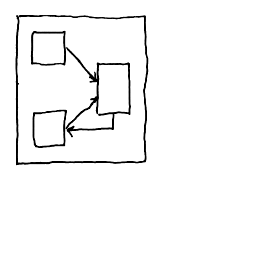
\includegraphics[width = 5cm]{../TikZ/drawings/expert-0.png}&
            
\includegraphics[width = 5cm]{../TikZ/drawings/expert-0-parses/0.png}&
    
        \begin{minipage}{10cm}
        \begin{verbatim}
line(6,2,3,2,arrow = True,solid = True);
line(6,2,6,3,arrow = False,solid = True);
rectangle(0,0,8,9);
rectangle(5,3,7,6);
reflect(reflect(y = 9)){
line(3,2,5,4,arrow = True,solid = True);
rectangle(1,6,3,8)
}
        \end{verbatim}
\end{minipage}

    \end{tabular}        
            \\

            \begin{tabular}{lll}
    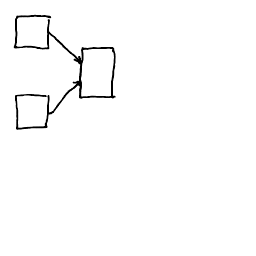
\includegraphics[width = 5cm]{../TikZ/drawings/expert-2.png}&
            
\includegraphics[width = 5cm]{../TikZ/drawings/expert-2-parses/0.png}&
    
        \begin{minipage}{10cm}
        \begin{verbatim}
rectangle(4,2,6,5);
reflect(reflect(y = 7)){
line(2,6,4,4,arrow = True,solid = True);
rectangle(0,5,2,7)
}
        \end{verbatim}
\end{minipage}

    \end{tabular}        
            \\

            \begin{tabular}{lll}
    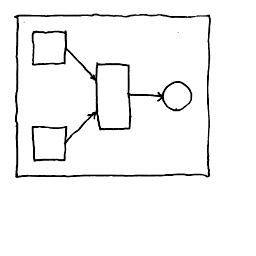
\includegraphics[width = 5cm]{../TikZ/drawings/expert-3.png}&
            
\includegraphics[width = 5cm]{../TikZ/drawings/expert-3-parses/0.png}&
    
        \begin{minipage}{10cm}
        \begin{verbatim}
circle(10,5);
line(7,5,9,5,arrow = True,solid = True);
rectangle(0,0,12,10);
reflect(reflect(y = 10)){
line(3,8,5,6,arrow = True,solid = True);
rectangle(1,1,3,3);
rectangle(5,3,7,7)
}
        \end{verbatim}
\end{minipage}

    \end{tabular}        
            \\

            \begin{tabular}{lll}
    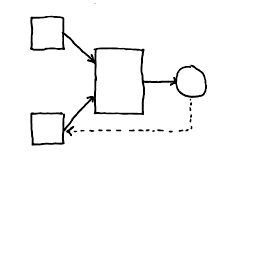
\includegraphics[width = 5cm]{../TikZ/drawings/expert-4.png}&
            
\includegraphics[width = 5cm]{../TikZ/drawings/expert-4-parses/0.png}&
    
        \begin{minipage}{10cm}
        \begin{verbatim}
circle(10,4);
line(10,1,10,3,arrow = False,solid = False);
line(10,1,2,1,arrow = True,solid = False);
line(7,4,9,4,arrow = True,solid = True);
reflect(reflect(y = 8)){
line(2,1,4,3,arrow = True,solid = True);
rectangle(0,6,2,8);
rectangle(4,2,7,6)
}
        \end{verbatim}
\end{minipage}

    \end{tabular}        
            \\

            \begin{tabular}{lll}
    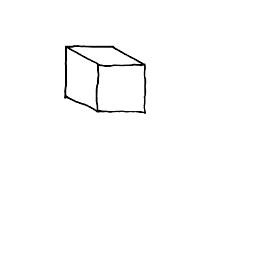
\includegraphics[width = 5cm]{../TikZ/drawings/expert-6.png}&
            
\includegraphics[width = 5cm]{../TikZ/drawings/expert-6-parses/0.png}&
    
        \begin{minipage}{10cm}
        \begin{verbatim}
rectangle(2,0,5,3);
for (i < 3){
if (i > 0){
line(0,3*i + -2,3*i + -3,4,arrow = False,solid = True);
line(3*i + -3,4,3*i + -1,3,arrow = False,solid = True)
}line(0,1,2,0,arrow = False,solid = True)
}
        \end{verbatim}
\end{minipage}

    \end{tabular}        
            \\

            \begin{tabular}{lll}
    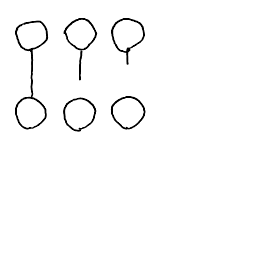
\includegraphics[width = 5cm]{../TikZ/drawings/expert-7.png}&
            
\includegraphics[width = 5cm]{../TikZ/drawings/expert-7-parses/0.png}&
    
        \begin{minipage}{10cm}
        \begin{verbatim}
for (i < 3){
circle(-3*i + 7,6);
circle(-3*i + 7,1);
line(-3*i + 7,-1*i + 4,-3*i + 7,5,arrow = False,solid = True)
}
        \end{verbatim}
\end{minipage}

    \end{tabular}        
            \\

            \begin{tabular}{lll}
    
\includegraphics[width = 5cm]{../TikZ/drawings/expert-8.png}&
            
\includegraphics[width = 5cm]{../TikZ/drawings/expert-8-parses/0.png}&
    
        \begin{minipage}{10cm}
        \begin{verbatim}
line(0,0,0,4,arrow = False,solid = True)
        \end{verbatim}
\end{minipage}

    \end{tabular}        
            \\

            \begin{tabular}{lll}
    
\includegraphics[width = 5cm]{../TikZ/drawings/expert-9.png}&
            
\includegraphics[width = 5cm]{../TikZ/drawings/expert-9-parses/0.png}&
    
        \begin{minipage}{10cm}
        \begin{verbatim}
line(6,0,0,0,arrow = True,solid = True)
        \end{verbatim}
\end{minipage}

    \end{tabular}        
            \\

            \begin{tabular}{lll}
    
\includegraphics[width = 5cm]{../TikZ/drawings/expert-10.png}&
            
\includegraphics[width = 5cm]{../TikZ/drawings/expert-10-parses/0.png}&
    
        \begin{minipage}{10cm}
        \begin{verbatim}
rectangle(0,0,3,4)
        \end{verbatim}
\end{minipage}

    \end{tabular}        
            \\

            \begin{tabular}{lll}
    
\includegraphics[width = 5cm]{../TikZ/drawings/expert-11.png}&
            
\includegraphics[width = 5cm]{../TikZ/drawings/expert-11-parses/0.png}&
    
        \begin{minipage}{10cm}
        \begin{verbatim}
circle(1,1)
        \end{verbatim}
\end{minipage}

    \end{tabular}        
            \\

            \begin{tabular}{lll}
    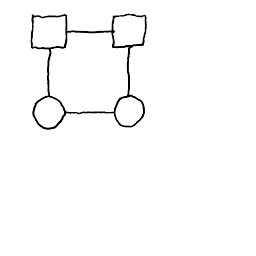
\includegraphics[width = 5cm]{../TikZ/drawings/expert-12.png}&
            
\includegraphics[width = 5cm]{../TikZ/drawings/expert-12-parses/0.png}&
    
        \begin{minipage}{10cm}
        \begin{verbatim}
line(2,1,5,1,arrow = False,solid = True);
reflect(reflect(x = 7)){
circle(1,1);
line(2,6,5,6,arrow = False,solid = True);
line(1,2,1,5,arrow = False,solid = True);
rectangle(0,5,2,7)
}
        \end{verbatim}
\end{minipage}

    \end{tabular}        
            \\

            \begin{tabular}{lll}
    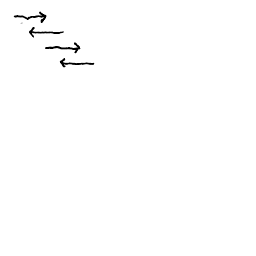
\includegraphics[width = 5cm]{../TikZ/drawings/expert-13.png}&
            
\includegraphics[width = 5cm]{../TikZ/drawings/expert-13-parses/0.png}&
    
        \begin{minipage}{10cm}
        \begin{verbatim}
line(3,2,1,2,arrow = True,solid = True);
line(5,0,3,0,arrow = True,solid = True);
line(2,1,4,1,arrow = True,solid = True);
line(0,3,2,3,arrow = True,solid = True)
        \end{verbatim}
\end{minipage}

    \end{tabular}        
            \\

            \begin{tabular}{lll}
    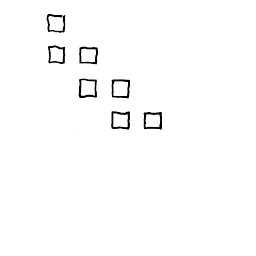
\includegraphics[width = 5cm]{../TikZ/drawings/expert-14.png}&
            
\includegraphics[width = 5cm]{../TikZ/drawings/expert-14-parses/0.png}&
    
        \begin{minipage}{10cm}
        \begin{verbatim}
for (i < 4){
if (i > 0){
rectangle(2*i + -2,-2*i + 6,2*i + -1,-2*i + 7)
}rectangle(2*i,-2*i + 6,2*i + 1,-2*i + 7)
}
        \end{verbatim}
\end{minipage}

    \end{tabular}        
            \\

            \begin{tabular}{lll}
    
\includegraphics[width = 5cm]{../TikZ/drawings/expert-15.png}&
            
\includegraphics[width = 5cm]{../TikZ/drawings/expert-15-parses/0.png}&
    
        \begin{minipage}{10cm}
        \begin{verbatim}
line(0,3,2,3,arrow = False,solid = False);
line(2,1,4,1,arrow = False,solid = False);
line(1,2,3,2,arrow = False,solid = True);
line(3,0,5,0,arrow = False,solid = True)
        \end{verbatim}
\end{minipage}

    \end{tabular}        
            \\

            \begin{tabular}{lll}
    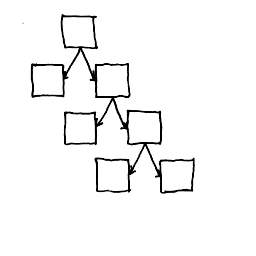
\includegraphics[width = 5cm]{../TikZ/drawings/expert-17.png}&
            
\includegraphics[width = 5cm]{../TikZ/drawings/expert-17-parses/0.png}&
    
        \begin{minipage}{10cm}
        \begin{verbatim}
for (i < 4){
if (i > 0){
line(-2*i + 9,3*i,-2*i + 10,3*i + -2,arrow = True,solid = True);
line(-2*i + 9,3*i,-2*i + 8,3*i + -2,arrow = True,solid = True);
rectangle(-2*i + 6,3*i + -3,-2*i + 8,3*i + -1)
}rectangle(-2*i + 8,3*i,-2*i + 10,3*i + 2)
}
        \end{verbatim}
\end{minipage}

    \end{tabular}        
            \\

            \begin{tabular}{lll}
    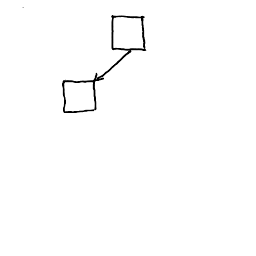
\includegraphics[width = 5cm]{../TikZ/drawings/expert-19.png}&
            
\includegraphics[width = 5cm]{../TikZ/drawings/expert-19-parses/0.png}&
    
        \begin{minipage}{10cm}
        \begin{verbatim}
line(4,4,2,2,arrow = True,solid = True);
rectangle(0,0,2,2);
rectangle(3,4,5,6)
        \end{verbatim}
\end{minipage}

    \end{tabular}        
            \\

            \begin{tabular}{lll}
    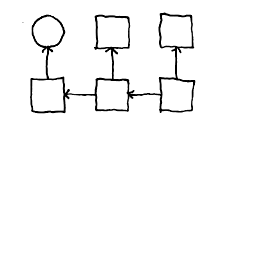
\includegraphics[width = 5cm]{../TikZ/drawings/expert-21.png}&
            
\includegraphics[width = 5cm]{../TikZ/drawings/expert-21-parses/0.png}&
    
        \begin{minipage}{10cm}
        \begin{verbatim}
circle(1,5);
for (i < 3){
if (i > 0){
line(-4*i + 12,1,-4*i + 10,1,arrow = True,solid = True);
rectangle(-4*i + 12,4,-4*i + 14,6)
}line(-4*i + 9,2,-4*i + 9,4,arrow = True,solid = True);
rectangle(-4*i + 8,0,-4*i + 10,2)
}
        \end{verbatim}
\end{minipage}

    \end{tabular}        
            \\

            \begin{tabular}{lll}
    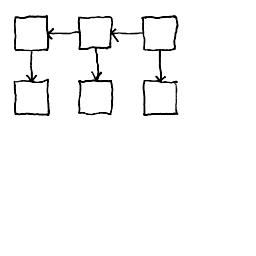
\includegraphics[width = 5cm]{../TikZ/drawings/expert-22.png}&
            
\includegraphics[width = 5cm]{../TikZ/drawings/expert-22-parses/0.png}&
    
        \begin{minipage}{10cm}
        \begin{verbatim}
for (i < 3){
if (i > 0){
line(4*i,5,4*i + -2,5,arrow = True,solid = True)
}line(4*i + 1,4,4*i + 1,2,arrow = True,solid = True);
rectangle(4*i,0,4*i + 2,2);
rectangle(4*i,4,4*i + 2,6)
}
        \end{verbatim}
\end{minipage}

    \end{tabular}        
            \\

            \begin{tabular}{lll}
    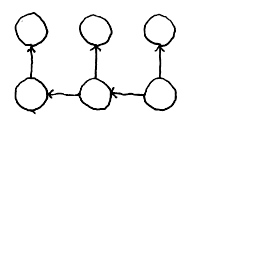
\includegraphics[width = 5cm]{../TikZ/drawings/expert-23.png}&
            
\includegraphics[width = 5cm]{../TikZ/drawings/expert-23-parses/0.png}&
    
        \begin{minipage}{10cm}
        \begin{verbatim}
for (i < 3){
line(-4*i + 9,2,-4*i + 9,4,arrow = True,solid = True);
for (j < 2){
circle(-4*i + 9,4*j + 1);
line(-4*j + 8,1,-4*j + 6,1,arrow = True,solid = True)
}
}
        \end{verbatim}
\end{minipage}

    \end{tabular}        
            \\

            \begin{tabular}{lll}
    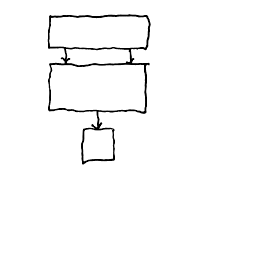
\includegraphics[width = 5cm]{../TikZ/drawings/expert-24.png}&
            
\includegraphics[width = 5cm]{../TikZ/drawings/expert-24-parses/0.png}&
    
        \begin{minipage}{10cm}
        \begin{verbatim}
reflect(reflect(x = 6)){
for (i < 3){
if (i > 0){
line(-2*i + 7,-4*i + 11,-2*i + 7,-4*i + 10,arrow = True,solid = True);
rectangle(0,-4*i + 11,6,-3*i + 12)
}rectangle(2,0,4,2)
}
}
        \end{verbatim}
\end{minipage}

    \end{tabular}        
            \\

            \begin{tabular}{lll}
    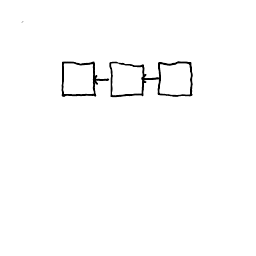
\includegraphics[width = 5cm]{../TikZ/drawings/expert-25.png}&
            
\includegraphics[width = 5cm]{../TikZ/drawings/expert-25-parses/0.png}&
    
        \begin{minipage}{10cm}
        \begin{verbatim}
for (i < 3){
if (i > 0){
line(-3*i + 9,1,-3*i + 8,1,arrow = True,solid = True)
}rectangle(-3*i + 6,0,-3*i + 8,2)
}
        \end{verbatim}
\end{minipage}

    \end{tabular}        
            \\

            \begin{tabular}{lll}
    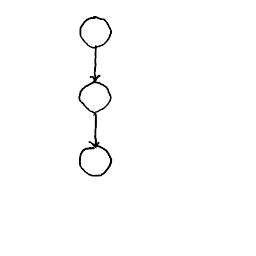
\includegraphics[width = 5cm]{../TikZ/drawings/expert-26.png}&
            
\includegraphics[width = 5cm]{../TikZ/drawings/expert-26-parses/0.png}&
    
        \begin{minipage}{10cm}
        \begin{verbatim}
line(1,3,1,4,arrow = False,solid = True);
for (i < 3){
if (i > 0){
line(1,-5*i + 13,1,-4*i + 10,arrow = True,solid = True)
}circle(1,-4*i + 9)
}
        \end{verbatim}
\end{minipage}

    \end{tabular}        
            \\

            \begin{tabular}{lll}
    
\includegraphics[width = 5cm]{../TikZ/drawings/expert-27.png}&
            
\includegraphics[width = 5cm]{../TikZ/drawings/expert-27-parses/0.png}&
    
        \begin{minipage}{10cm}
        \begin{verbatim}
reflect(reflect(x = 2)){
line(0,1,1,2,arrow = False,solid = True);
line(1,0,2,1,arrow = False,solid = True)
}
        \end{verbatim}
\end{minipage}

    \end{tabular}        
            \\

            \begin{tabular}{lll}
    
\includegraphics[width = 5cm]{../TikZ/drawings/expert-28.png}&
            
\includegraphics[width = 5cm]{../TikZ/drawings/expert-28-parses/0.png}&
    
        \begin{minipage}{10cm}
        \begin{verbatim}
line(0,2,2,2,arrow = False,solid = True);
line(0,0,0,2,arrow = False,solid = True)
        \end{verbatim}
\end{minipage}

    \end{tabular}        
            \\

            \begin{tabular}{lll}
    
\includegraphics[width = 5cm]{../TikZ/drawings/expert-29.png}&
            
\includegraphics[width = 5cm]{../TikZ/drawings/expert-29-parses/0.png}&
    
        \begin{minipage}{10cm}
        \begin{verbatim}
for (i < 3){
line(-1*i + 2,i + 4,-2*i + 6,i + 4,arrow = False,solid = True);
line(-1*i + 2,2*i,-1*i + 2,i + 4,arrow = False,solid = True)
}
        \end{verbatim}
\end{minipage}

    \end{tabular}        
            \\

            \begin{tabular}{lll}
    \includegraphics[width = 5cm]{../TikZ/drawings/expert-30.png}&
            \includegraphics[width = 5cm]{../TikZ/drawings/expert-30-parses/0.png}&
    
        \begin{minipage}{10cm}
        \begin{verbatim}
for (i < 3){
if (i > 0){
circle(5,2*i);
circle(1,-3*i + 7);
rectangle(0,-3*i + 6,2,-3*i + 8)
}rectangle(4,1,6,5)
}
        \end{verbatim}
\end{minipage}

    \end{tabular}        
            \\

            \begin{tabular}{lll}
    \includegraphics[width = 5cm]{../TikZ/drawings/expert-31.png}&
            \includegraphics[width = 5cm]{../TikZ/drawings/expert-31-parses/0.png}&
    
        \begin{minipage}{10cm}
        \begin{verbatim}
for (i < 3){
rectangle(3*i,-2*i + 4,3*i + 2,6);
for (j < i + 1){
circle(3*i + 1,-2*j + 5)
}
}
        \end{verbatim}
\end{minipage}

    \end{tabular}        
            \\

            \begin{tabular}{lll}
    \includegraphics[width = 5cm]{../TikZ/drawings/expert-32.png}&
            \includegraphics[width = 5cm]{../TikZ/drawings/expert-32-parses/0.png}&
    
        \begin{minipage}{10cm}
        \begin{verbatim}
circle(5,5);
line(2,5,4,5,arrow = False,solid = True);
rectangle(0,0,5,3);
rectangle(0,4,2,6)
        \end{verbatim}
\end{minipage}

    \end{tabular}        
            \\

            \begin{tabular}{lll}
    \includegraphics[width = 5cm]{../TikZ/drawings/expert-33.png}&
            \includegraphics[width = 5cm]{../TikZ/drawings/expert-33-parses/0.png}&
    
        \begin{minipage}{10cm}
        \begin{verbatim}
line(0,0,6,0,arrow = False,solid = False);
line(0,3,6,3,arrow = False,solid = False);
line(6,0,6,3,arrow = False,solid = True);
line(0,0,0,3,arrow = False,solid = True)
        \end{verbatim}
\end{minipage}

    \end{tabular}        
            \\

            \begin{tabular}{lll}
    \includegraphics[width = 5cm]{../TikZ/drawings/expert-35.png}&
            \includegraphics[width = 5cm]{../TikZ/drawings/expert-35-parses/0.png}&
    
        \begin{minipage}{10cm}
        \begin{verbatim}
for (i < 3){
if (i > 0){
circle(5*i + -4,1);
line(i,i + 4,5*i + -4,2,arrow = True,solid = True)
}circle(1,6)
}
        \end{verbatim}
\end{minipage}

    \end{tabular}        
            \\

            \begin{tabular}{lll}
    \includegraphics[width = 5cm]{../TikZ/drawings/expert-37.png}&
            \includegraphics[width = 5cm]{../TikZ/drawings/expert-37-parses/0.png}&
    
        \begin{minipage}{10cm}
        \begin{verbatim}
for (i < 3){
if (i > 0){
line(-4*i + 9,5*i + -3,-2*i + 7,5,arrow = False,solid = True);
rectangle(-4*i + 8,5*i + -5,6,7*i + -5)
}circle(1,8)
}
        \end{verbatim}
\end{minipage}

    \end{tabular}        
            \\

            \begin{tabular}{lll}
    \includegraphics[width = 5cm]{../TikZ/drawings/expert-40.png}&
            \includegraphics[width = 5cm]{../TikZ/drawings/expert-40-parses/0.png}&
    
        \begin{minipage}{10cm}
        \begin{verbatim}
for (i < 3){
circle(3*i + 1,1)
}
        \end{verbatim}
\end{minipage}

    \end{tabular}        
            \\

            \begin{tabular}{lll}
    \includegraphics[width = 5cm]{../TikZ/drawings/expert-41.png}&
            \includegraphics[width = 5cm]{../TikZ/drawings/expert-41-parses/0.png}&
    
        \begin{minipage}{10cm}
        \begin{verbatim}
for (i < 3){
rectangle(2*i,0,2*i + 1,6)
}
        \end{verbatim}
\end{minipage}

    \end{tabular}        
            \\

            \begin{tabular}{lll}
    \includegraphics[width = 5cm]{../TikZ/drawings/expert-42.png}&
            \includegraphics[width = 5cm]{../TikZ/drawings/expert-42-parses/0.png}&
    
        \begin{minipage}{10cm}
        \begin{verbatim}
line(0,0,0,5,arrow = False,solid = False);
line(4,1,4,5,arrow = False,solid = False);
line(4,0,4,1,arrow = False,solid = False)
        \end{verbatim}
\end{minipage}

    \end{tabular}        
            \\

            \begin{tabular}{lll}
    \includegraphics[width = 5cm]{../TikZ/drawings/expert-43.png}&
            \includegraphics[width = 5cm]{../TikZ/drawings/expert-43-parses/0.png}&
    
        \begin{minipage}{10cm}
        \begin{verbatim}
line(0,0,0,5,arrow = False,solid = True);
line(4,0,4,5,arrow = False,solid = True)
        \end{verbatim}
\end{minipage}

    \end{tabular}        
            \\

            \begin{tabular}{lll}
    \includegraphics[width = 5cm]{../TikZ/drawings/expert-44.png}&
            \includegraphics[width = 5cm]{../TikZ/drawings/expert-44-parses/0.png}&
    
        \begin{minipage}{10cm}
        \begin{verbatim}
reflect(reflect(x = 12)){
circle(4,1);
line(9,1,10,1,arrow = False,solid = True);
rectangle(10,0,12,2)
}
        \end{verbatim}
\end{minipage}

    \end{tabular}        
            \\

            \begin{tabular}{lll}
    \includegraphics[width = 5cm]{../TikZ/drawings/expert-45.png}&
            \includegraphics[width = 5cm]{../TikZ/drawings/expert-45-parses/0.png}&
    
        \begin{minipage}{10cm}
        \begin{verbatim}
line(4,6,6,6,arrow = True,solid = True);
rectangle(0,4,4,8);
reflect(reflect(y = 12)){
circle(7,6);
line(2,10,2,8,arrow = True,solid = True);
rectangle(1,0,3,2)
}
        \end{verbatim}
\end{minipage}

    \end{tabular}        
            \\

            \begin{tabular}{lll}
    \includegraphics[width = 5cm]{../TikZ/drawings/expert-46.png}&
            \includegraphics[width = 5cm]{../TikZ/drawings/expert-46-parses/0.png}&
    
        \begin{minipage}{10cm}
        \begin{verbatim}
reflect(reflect(x = 9)){
line(1,3,1,6,arrow = False,solid = True);
reflect(reflect(y = 9)){
circle(1,8);
line(3,1,6,1,arrow = False,solid = True)
}
}
        \end{verbatim}
\end{minipage}

    \end{tabular}        
            \\

            \begin{tabular}{lll}
    \includegraphics[width = 5cm]{../TikZ/drawings/expert-47.png}&
            \includegraphics[width = 5cm]{../TikZ/drawings/expert-47-parses/0.png}&
    
        \begin{minipage}{10cm}
        \begin{verbatim}
reflect(reflect(y = 11)){
rectangle(4,1,7,2);
reflect(reflect(x = 11)){
rectangle(1,4,2,7);
rectangle(0,8,3,11)
}
}
        \end{verbatim}
\end{minipage}

    \end{tabular}        
            \\

            \begin{tabular}{lll}
    \includegraphics[width = 5cm]{../TikZ/drawings/expert-48.png}&
            \includegraphics[width = 5cm]{../TikZ/drawings/expert-48-parses/0.png}&
    
        \begin{minipage}{10cm}
        \begin{verbatim}
for (i < 3){
line(-2*i + 5,2*i,-2*i + 7,2*i,arrow = False,solid = True);
line(-2*i + 4,2*i + 1,-2*i + 6,2*i + 1,arrow = False,solid = True)
}
        \end{verbatim}
\end{minipage}

    \end{tabular}        
            \\

            \begin{tabular}{lll}
    \includegraphics[width = 5cm]{../TikZ/drawings/expert-49.png}&
            \includegraphics[width = 5cm]{../TikZ/drawings/expert-49-parses/0.png}&
    
        \begin{minipage}{10cm}
        \begin{verbatim}
for (i < 3){
if (i > 0){
rectangle(-3*i + 10,i + -1,-3*i + 12,2);
rectangle(0,-7*i + 14,3,-7*i + 17)
}rectangle(1,4,2,6)
}
        \end{verbatim}
\end{minipage}

    \end{tabular}        
            \\

            \begin{tabular}{lll}
    \includegraphics[width = 5cm]{../TikZ/drawings/expert-51.png}&
            \includegraphics[width = 5cm]{../TikZ/drawings/expert-51-parses/0.png}&
    
        \begin{minipage}{10cm}
        \begin{verbatim}
for (i < 3){
rectangle(2*i,2*i,2*i + 3,2*i + 1)
}
        \end{verbatim}
\end{minipage}

    \end{tabular}        
            \\

            \begin{tabular}{lll}
    \includegraphics[width = 5cm]{../TikZ/drawings/expert-52.png}&
            \includegraphics[width = 5cm]{../TikZ/drawings/expert-52-parses/0.png}&
    
        \begin{minipage}{10cm}
        \begin{verbatim}
circle(4,10);
for (i < 3){
circle(3*i + 1,5);
circle(3*i + 1,1);
line(4,9,3*i + 1,6,arrow = True,solid = True);
line(3*i + 1,4,3*i + 1,2,arrow = True,solid = True)
}
        \end{verbatim}
\end{minipage}

    \end{tabular}        
            \\

            \begin{tabular}{lll}
    \includegraphics[width = 5cm]{../TikZ/drawings/expert-53.png}&
            \includegraphics[width = 5cm]{../TikZ/drawings/expert-53-parses/0.png}&
    
        \begin{minipage}{10cm}
        \begin{verbatim}
line(6,8,6,4,arrow = True,solid = True);
line(0,8,8,8,arrow = False,solid = True);
line(4,8,4,0,arrow = True,solid = True);
line(2,8,2,6,arrow = True,solid = True)
        \end{verbatim}
\end{minipage}

    \end{tabular}        
            \\

            \begin{tabular}{lll}
    \includegraphics[width = 5cm]{../TikZ/drawings/expert-54.png}&
            \includegraphics[width = 5cm]{../TikZ/drawings/expert-54-parses/0.png}&
    
        \begin{minipage}{10cm}
        \begin{verbatim}
line(2,3,2,5,arrow = False,solid = True);
rectangle(0,0,4,8);
reflect(reflect(y = 8)){
rectangle(1,5,3,7)
}
        \end{verbatim}
\end{minipage}

    \end{tabular}        
            \\

            \begin{tabular}{lll}
    \includegraphics[width = 5cm]{../TikZ/drawings/expert-55.png}&
            \includegraphics[width = 5cm]{../TikZ/drawings/expert-55-parses/0.png}&
    
        \begin{minipage}{10cm}
        \begin{verbatim}
circle(1,5);
line(1,4,1,2,arrow = True,solid = True);
rectangle(0,0,2,2)
        \end{verbatim}
\end{minipage}

    \end{tabular}        
            \\

            \begin{tabular}{lll}
    \includegraphics[width = 5cm]{../TikZ/drawings/expert-57.png}&
            \includegraphics[width = 5cm]{../TikZ/drawings/expert-57-parses/0.png}&
    
        \begin{minipage}{10cm}
        \begin{verbatim}
for (i < 3){
for (j < 3){
circle(-4*i + 9,-3*j + 7)
}
}
        \end{verbatim}
\end{minipage}

    \end{tabular}        
            \\

            \begin{tabular}{lll}
    \includegraphics[width = 5cm]{../TikZ/drawings/expert-58.png}&
            \includegraphics[width = 5cm]{../TikZ/drawings/expert-58-parses/0.png}&
    
        \begin{minipage}{10cm}
        \begin{verbatim}
for (i < 3){
if (i > 0){
line(8,0,8*i + -8,7*i + -7,arrow = True,solid = True)
}rectangle(-2*i + 6,0,-2*i + 7,-1*i + 5)
}
        \end{verbatim}
\end{minipage}

    \end{tabular}        
            \\

            \begin{tabular}{lll}
    \includegraphics[width = 5cm]{../TikZ/drawings/expert-59.png}&
            \includegraphics[width = 5cm]{../TikZ/drawings/expert-59-parses/0.png}&
    
        \begin{minipage}{10cm}
        \begin{verbatim}
line(4,0,0,0,arrow = False,solid = False)
        \end{verbatim}
\end{minipage}

    \end{tabular}        
            \\

            \begin{tabular}{lll}
    \includegraphics[width = 5cm]{../TikZ/drawings/expert-61.png}&
            \includegraphics[width = 5cm]{../TikZ/drawings/expert-61-parses/0.png}&
    
        \begin{minipage}{10cm}
        \begin{verbatim}
circle(2,1);
circle(6,1);
line(5,1,3,1,arrow = True,solid = True);
rectangle(0,0,7,2)
        \end{verbatim}
\end{minipage}

    \end{tabular}        
            \\

            \begin{tabular}{lll}
    \includegraphics[width = 5cm]{../TikZ/drawings/expert-62.png}&
            \includegraphics[width = 5cm]{../TikZ/drawings/expert-62-parses/0.png}&
    
        \begin{minipage}{10cm}
        \begin{verbatim}
rectangle(5,0,8,3);
rectangle(0,2,1,3);
rectangle(2,1,4,3)
        \end{verbatim}
\end{minipage}

    \end{tabular}        
            \\

            \begin{tabular}{lll}
    \includegraphics[width = 5cm]{../TikZ/drawings/expert-63.png}&
            \includegraphics[width = 5cm]{../TikZ/drawings/expert-63-parses/0.png}&
    
        \begin{minipage}{10cm}
        \begin{verbatim}
for (i < 3){
rectangle(i,i,-1*i + 5,-1*i + 5)
}
        \end{verbatim}
\end{minipage}

    \end{tabular}        
            \\

            \begin{tabular}{lll}
    \includegraphics[width = 5cm]{../TikZ/drawings/expert-64.png}&
            \includegraphics[width = 5cm]{../TikZ/drawings/expert-64-parses/0.png}&
    
        \begin{minipage}{10cm}
        \begin{verbatim}
reflect(reflect(x = 6)){
line(5,2,5,4,arrow = False,solid = True);
reflect(reflect(y = 6)){
line(2,1,4,1,arrow = False,solid = True);
rectangle(4,4,6,6)
}
}
        \end{verbatim}
\end{minipage}

    \end{tabular}        
            \\

            \begin{tabular}{lll}
    \includegraphics[width = 5cm]{../TikZ/drawings/expert-65.png}&
            \includegraphics[width = 5cm]{../TikZ/drawings/expert-65-parses/0.png}&
    
        \begin{minipage}{10cm}
        \begin{verbatim}
reflect(reflect(x = 6)){
line(1,2,1,4,arrow = False,solid = True);
reflect(reflect(y = 6)){
circle(5,1);
line(2,1,4,1,arrow = False,solid = True)
}
}
        \end{verbatim}
\end{minipage}

    \end{tabular}        
            \\

            \begin{tabular}{lll}
    \includegraphics[width = 5cm]{../TikZ/drawings/expert-66.png}&
            \includegraphics[width = 5cm]{../TikZ/drawings/expert-66-parses/0.png}&
    
        \begin{minipage}{10cm}
        \begin{verbatim}
for (i < 3){
line(i,-1*i + 2,-1*i + 7,-1*i + 2,arrow = False,solid = True)
}
        \end{verbatim}
\end{minipage}

    \end{tabular}        
            \\

            \begin{tabular}{lll}
    \includegraphics[width = 5cm]{../TikZ/drawings/expert-67.png}&
            \includegraphics[width = 5cm]{../TikZ/drawings/expert-67-parses/0.png}&
    
        \begin{minipage}{10cm}
        \begin{verbatim}
line(1,4,5,0,arrow = False,solid = True);
line(1,5,5,1,arrow = False,solid = True);
rectangle(0,4,1,5);
rectangle(5,0,6,1)
        \end{verbatim}
\end{minipage}

    \end{tabular}        
            \\

            \begin{tabular}{lll}
    \includegraphics[width = 5cm]{../TikZ/drawings/expert-68.png}&
            \includegraphics[width = 5cm]{../TikZ/drawings/expert-68-parses/0.png}&
    
        \begin{minipage}{10cm}
        \begin{verbatim}
for (i < 3){
circle(4*i + 1,1);
rectangle(4*i,0,4*i + 2,2)
}
        \end{verbatim}
\end{minipage}

    \end{tabular}        
            \\

            \begin{tabular}{lll}
    \includegraphics[width = 5cm]{../TikZ/drawings/expert-69.png}&
            \includegraphics[width = 5cm]{../TikZ/drawings/expert-69-parses/0.png}&
    
        \begin{minipage}{10cm}
        \begin{verbatim}
rectangle(0,4,5,6);
reflect(reflect(x = 5)){
circle(1,1);
line(1,4,1,2,arrow = True,solid = True)
}
        \end{verbatim}
\end{minipage}

    \end{tabular}        
            \\

            \begin{tabular}{lll}
    \includegraphics[width = 5cm]{../TikZ/drawings/expert-70.png}&
            \includegraphics[width = 5cm]{../TikZ/drawings/expert-70-parses/0.png}&
    
        \begin{minipage}{10cm}
        \begin{verbatim}
reflect(reflect(x = 6)){
circle(1,9);
for (i < 3){
if (i > 0){
circle(-2*i + 7,-4*i + 9);
line(5,-4*i + 12,-2*i + 7,-4*i + 10,arrow = True,solid = True)
}line(1,8,4,5,arrow = True,solid = True)
}
}
        \end{verbatim}
\end{minipage}

    \end{tabular}        
            \\

            \begin{tabular}{lll}
    \includegraphics[width = 5cm]{../TikZ/drawings/expert-72.png}&
            \includegraphics[width = 5cm]{../TikZ/drawings/expert-72-parses/0.png}&
    
        \begin{minipage}{10cm}
        \begin{verbatim}
reflect(reflect(y = 8)){
for (i < 3){
if (i > 0){
rectangle(3*i + -1,-3*i + 8,3*i,-3*i + 9)
}circle(3*i + 1,-3*i + 7)
}
}
        \end{verbatim}
\end{minipage}

    \end{tabular}        
            \\

            \begin{tabular}{lll}
    \includegraphics[width = 5cm]{../TikZ/drawings/expert-74.png}&
            \includegraphics[width = 5cm]{../TikZ/drawings/expert-74-parses/0.png}&
    
        \begin{minipage}{10cm}
        \begin{verbatim}
for (i < 3){
if (i > 0){
rectangle(2*i + -2,2*i + -2,-2*i + 8,-2*i + 8)
}for (j < 3){
circle(2*j + 1,2*i + 1)
}
}
        \end{verbatim}
\end{minipage}

    \end{tabular}        
            \\

            \begin{tabular}{lll}
    \includegraphics[width = 5cm]{../TikZ/drawings/expert-75.png}&
            \includegraphics[width = 5cm]{../TikZ/drawings/expert-75-parses/0.png}&
    
        \begin{minipage}{10cm}
        \begin{verbatim}
for (i < 4){
line(-4*i + 13,4,-4*i + 13,2,arrow = True,solid = True);
for (j < 3){
if (j > 0){
circle(-4*i + 13,-4*j + 9)
}line(-4*j + 10,5,-4*j + 12,5,arrow = True,solid = True)
}
}
        \end{verbatim}
\end{minipage}

    \end{tabular}        
            \\

            \begin{tabular}{lll}
    \includegraphics[width = 5cm]{../TikZ/drawings/expert-76.png}&
            \includegraphics[width = 5cm]{../TikZ/drawings/expert-76-parses/0.png}&
    
        \begin{minipage}{10cm}
        \begin{verbatim}
line(4,5,4,10,arrow = False,solid = True);
reflect(reflect(x = 8)){
circle(4,1);
circle(1,8);
line(4,5,8,2,arrow = False,solid = True)
}
        \end{verbatim}
\end{minipage}

    \end{tabular}        
            \\

            \begin{tabular}{lll}
    \includegraphics[width = 5cm]{../TikZ/drawings/expert-78.png}&
            \includegraphics[width = 5cm]{../TikZ/drawings/expert-78-parses/0.png}&
    
        \begin{minipage}{10cm}
        \begin{verbatim}
line(0,6,12,6,arrow = False,solid = True);
line(8,3,7,4,arrow = True,solid = True);
line(3,2,5,4,arrow = True,solid = True);
line(6,6,6,5,arrow = True,solid = True);
reflect(reflect(x = 12)){
line(4,0,12,8,arrow = False,solid = True)
}
        \end{verbatim}
\end{minipage}

    \end{tabular}        
            \\

            \begin{tabular}{lll}
    \includegraphics[width = 5cm]{../TikZ/drawings/expert-81.png}&
            \includegraphics[width = 5cm]{../TikZ/drawings/expert-81-parses/0.png}&
    
        \begin{minipage}{10cm}
        \begin{verbatim}
circle(1,1);
circle(4,1);
rectangle(9,0,11,2);
rectangle(6,0,8,2)
        \end{verbatim}
\end{minipage}

    \end{tabular}        
            \\

            \begin{tabular}{lll}
    \includegraphics[width = 5cm]{../TikZ/drawings/expert-85.png}&
            \includegraphics[width = 5cm]{../TikZ/drawings/expert-85-parses/0.png}&
    
        \begin{minipage}{10cm}
        \begin{verbatim}
for (i < 4){
if (i > 0){
line(1,-3*i + 12,1,-3*i + 11,arrow = True,solid = True)
}circle(1,-3*i + 10)
}
        \end{verbatim}
\end{minipage}

    \end{tabular}        
            \\

            \begin{tabular}{lll}
    \includegraphics[width = 5cm]{../TikZ/drawings/expert-87.png}&
            \includegraphics[width = 5cm]{../TikZ/drawings/expert-87-parses/0.png}&
    
        \begin{minipage}{10cm}
        \begin{verbatim}
reflect(reflect(x = 8)){
rectangle(0,0,1,1);
rectangle(0,5,3,8);
rectangle(0,2,2,4)
}
        \end{verbatim}
\end{minipage}

    \end{tabular}        
            \\

            \begin{tabular}{lll}
    \includegraphics[width = 5cm]{../TikZ/drawings/expert-88.png}&
            \includegraphics[width = 5cm]{../TikZ/drawings/expert-88-parses/0.png}&
    
        \begin{minipage}{10cm}
        \begin{verbatim}
for (i < 3){
rectangle(2*i,i,-1*i + 8,-2*i + 7)
}
        \end{verbatim}
\end{minipage}

    \end{tabular}        
            \\

            \begin{tabular}{lll}
    \includegraphics[width = 5cm]{../TikZ/drawings/expert-90.png}&
            \includegraphics[width = 5cm]{../TikZ/drawings/expert-90-parses/0.png}&
    
        \begin{minipage}{10cm}
        \begin{verbatim}
circle(6,2);
line(6,6,6,3,arrow = True,solid = True);
rectangle(4,0,8,9);
for (i < 3){
if (i > 0){
line(-5*i + 15,7,-5*i + 12,7,arrow = True,solid = True)
}circle(-5*i + 11,7)
}
        \end{verbatim}
\end{minipage}

    \end{tabular}        
            \\

            \begin{tabular}{lll}
    \includegraphics[width = 5cm]{../TikZ/drawings/expert-91.png}&
            \includegraphics[width = 5cm]{../TikZ/drawings/expert-91-parses/0.png}&
    
        \begin{minipage}{10cm}
        \begin{verbatim}
reflect(reflect(y = 5)){
reflect(reflect(x = 5)){
line(0,0,2,0,arrow = False,solid = True);
line(0,0,0,2,arrow = False,solid = True)
}
}
        \end{verbatim}
\end{minipage}

    \end{tabular}        
            \\

            \begin{tabular}{lll}
    \includegraphics[width = 5cm]{../TikZ/drawings/expert-92.png}&
            \includegraphics[width = 5cm]{../TikZ/drawings/expert-92-parses/0.png}&
    
        \begin{minipage}{10cm}
        \begin{verbatim}
reflect(reflect(x = 14)){
for (i < 3){
circle(5,-4*i + 9);
line(10,-4*i + 9,12,-4*i + 9,arrow = False,solid = True);
rectangle(12,-4*i + 8,14,-4*i + 10)
}
}
        \end{verbatim}
\end{minipage}

    \end{tabular}        
            \\

            \begin{tabular}{lll}
    \includegraphics[width = 5cm]{../TikZ/drawings/expert-93.png}&
            \includegraphics[width = 5cm]{../TikZ/drawings/expert-93-parses/0.png}&
    
        \begin{minipage}{10cm}
        \begin{verbatim}
reflect(reflect(x = 10)){
for (i < 3){
if (i > 0){
line(-4*i + 13,4*i + -2,-4*i + 9,4*i,arrow = True,solid = True)
}circle(-4*i + 9,4*i + 1)
}
}
        \end{verbatim}
\end{minipage}

    \end{tabular}        
            \\

            \begin{tabular}{lll}
    \includegraphics[width = 5cm]{../TikZ/drawings/expert-94.png}&
            \includegraphics[width = 5cm]{../TikZ/drawings/expert-94-parses/0.png}&
    
        \begin{minipage}{10cm}
        \begin{verbatim}
line(0,2,12,2,arrow = False,solid = True);
line(6,2,6,3,arrow = True,solid = True);
reflect(reflect(x = 12)){
line(0,0,9,9,arrow = False,solid = True);
line(10,7,7,4,arrow = True,solid = True)
}
        \end{verbatim}
\end{minipage}

    \end{tabular}        
            \\

            \begin{tabular}{lll}
    \includegraphics[width = 5cm]{../TikZ/drawings/expert-95.png}&
            \includegraphics[width = 5cm]{../TikZ/drawings/expert-95-parses/0.png}&
    
        \begin{minipage}{10cm}
        \begin{verbatim}
circle(4,1);
reflect(reflect(x = 8)){
for (i < 3){
if (i > 0){
circle(1,-5*i + 16);
line(1,10,6*i + -5,7,arrow = True,solid = True)
}line(7,5,4,2,arrow = True,solid = True)
}
}
        \end{verbatim}
\end{minipage}

    \end{tabular}        
            \\

            \begin{tabular}{lll}
    \includegraphics[width = 5cm]{../TikZ/drawings/expert-96.png}&
            \includegraphics[width = 5cm]{../TikZ/drawings/expert-96-parses/0.png}&
    
        \begin{minipage}{10cm}
        \begin{verbatim}
reflect(reflect(x = 10)){
circle(9,1);
for (i < 4){
circle(-2*i + 7,2*i + 3)
}
}
        \end{verbatim}
\end{minipage}

    \end{tabular}        
            \\

            \begin{tabular}{lll}
    \includegraphics[width = 5cm]{../TikZ/drawings/expert-97.png}&
            \includegraphics[width = 5cm]{../TikZ/drawings/expert-97-parses/0.png}&
    
        \begin{minipage}{10cm}
        \begin{verbatim}
reflect(reflect(x = 6)){
for (i < 3){
if (i > 0){
line(1,-4*i + 10,1,-4*i + 12,arrow = False,solid = True)
}circle(1,-4*i + 9);
line(2,-4*i + 9,4,-4*i + 9,arrow = False,solid = True)
}
}
        \end{verbatim}
\end{minipage}

    \end{tabular}        
            \\

            \begin{tabular}{lll}
    \includegraphics[width = 5cm]{../TikZ/drawings/expert-98.png}&
            \includegraphics[width = 5cm]{../TikZ/drawings/expert-98-parses/0.png}&
    
        \begin{minipage}{10cm}
        \begin{verbatim}
rectangle(0,0,4,9);
for (i < 3){
if (i > 0){
circle(2,-4*i + 10);
line(2,-5*i + 15,2,-4*i + 11,arrow = True,solid = True)
}circle(2,11)
}
        \end{verbatim}
\end{minipage}

    \end{tabular}        
            \\

            \begin{tabular}{lll}
    \includegraphics[width = 5cm]{../TikZ/drawings/expert-99.png}&
            \includegraphics[width = 5cm]{../TikZ/drawings/expert-99-parses/0.png}&
    
        \begin{minipage}{10cm}
        \begin{verbatim}
for (i < 2){
circle(4,6*i + 1);
circle(1,6*i + 4);
rectangle(3,6*i + 3,5,6*i + 5);
rectangle(0,6*i,2,6*i + 2)
}
        \end{verbatim}
\end{minipage}

    \end{tabular}        
            